\section{Method}
\label{ch4:sec:method}
The proposed models utilize deep geometric learning to offer flexible CFD mesh parameterization.
They are designed to encode a target shape and then deform a given CFD mesh built on a fixed shape template to reconstruct the target geometry. Only points sampled on the target's surface are fed into the pipeline, which then generates an entire CFD mesh by inferring the model.
The pipelines of LSM and DMM are shown in Fig.\ref{ch4:fig:framework_LSM} and Fig.\ref{ch4:fig:framework_DMM}, respectively.

To formalize this process, we consider a 2D template airfoil with two sets of sampled points: $\hat{V}^S = \{\hat{\bv}^S_1, \hat{\bv}^S_2,..., \hat{\bv}^S_n$\} on the surface and $\hat{V}^V = \{\hat{\bv}^V_1, \hat{\bv}^V_2,..., \hat{\bv}^V_m$\} from its surrounding CFD computational domain, respectively. The sampling sizes can be arbitrary. The same vertices in a deformed continuous coordinate space can be represented as $V=\hat{V}+\Delta V$, where $\Delta V = \{\delta {\bv}_1, \delta {\bv}_2,...\}$ is the displacement vector of vertices.
During training, we compute the difference between the $O$ points sampled from the surface of the target airfoil to be parameterized, as denoted by $S=\{\textbf{s}_1, \textbf{s}_2,..., \textbf{s}_o\}$, and $\hat{V}^S$ as the supervised loss, while using $\hat{V}^V$ for unsupervised optimization in the regularization loss.
At the inference stage, $\hat{V}^S$ and $\hat{V}^V$ are resampled according to a user-defined CFD mesh $\hat{M}={\{\hat{V}^S, \hat{V}^V}, \hat{E}\}$ where $\hat{E}$ defines the edges connecting all vertices. Both LSM and DMM perform mesh deformation and infer a deformed CFD mesh $M={\{\hat{V}^S + \Delta V^S, \hat{V}^V + \Delta V^V}, \hat{E}\}$ with the mesh topology fixed.

\begin{figure}[tb]
    \begin{center}
        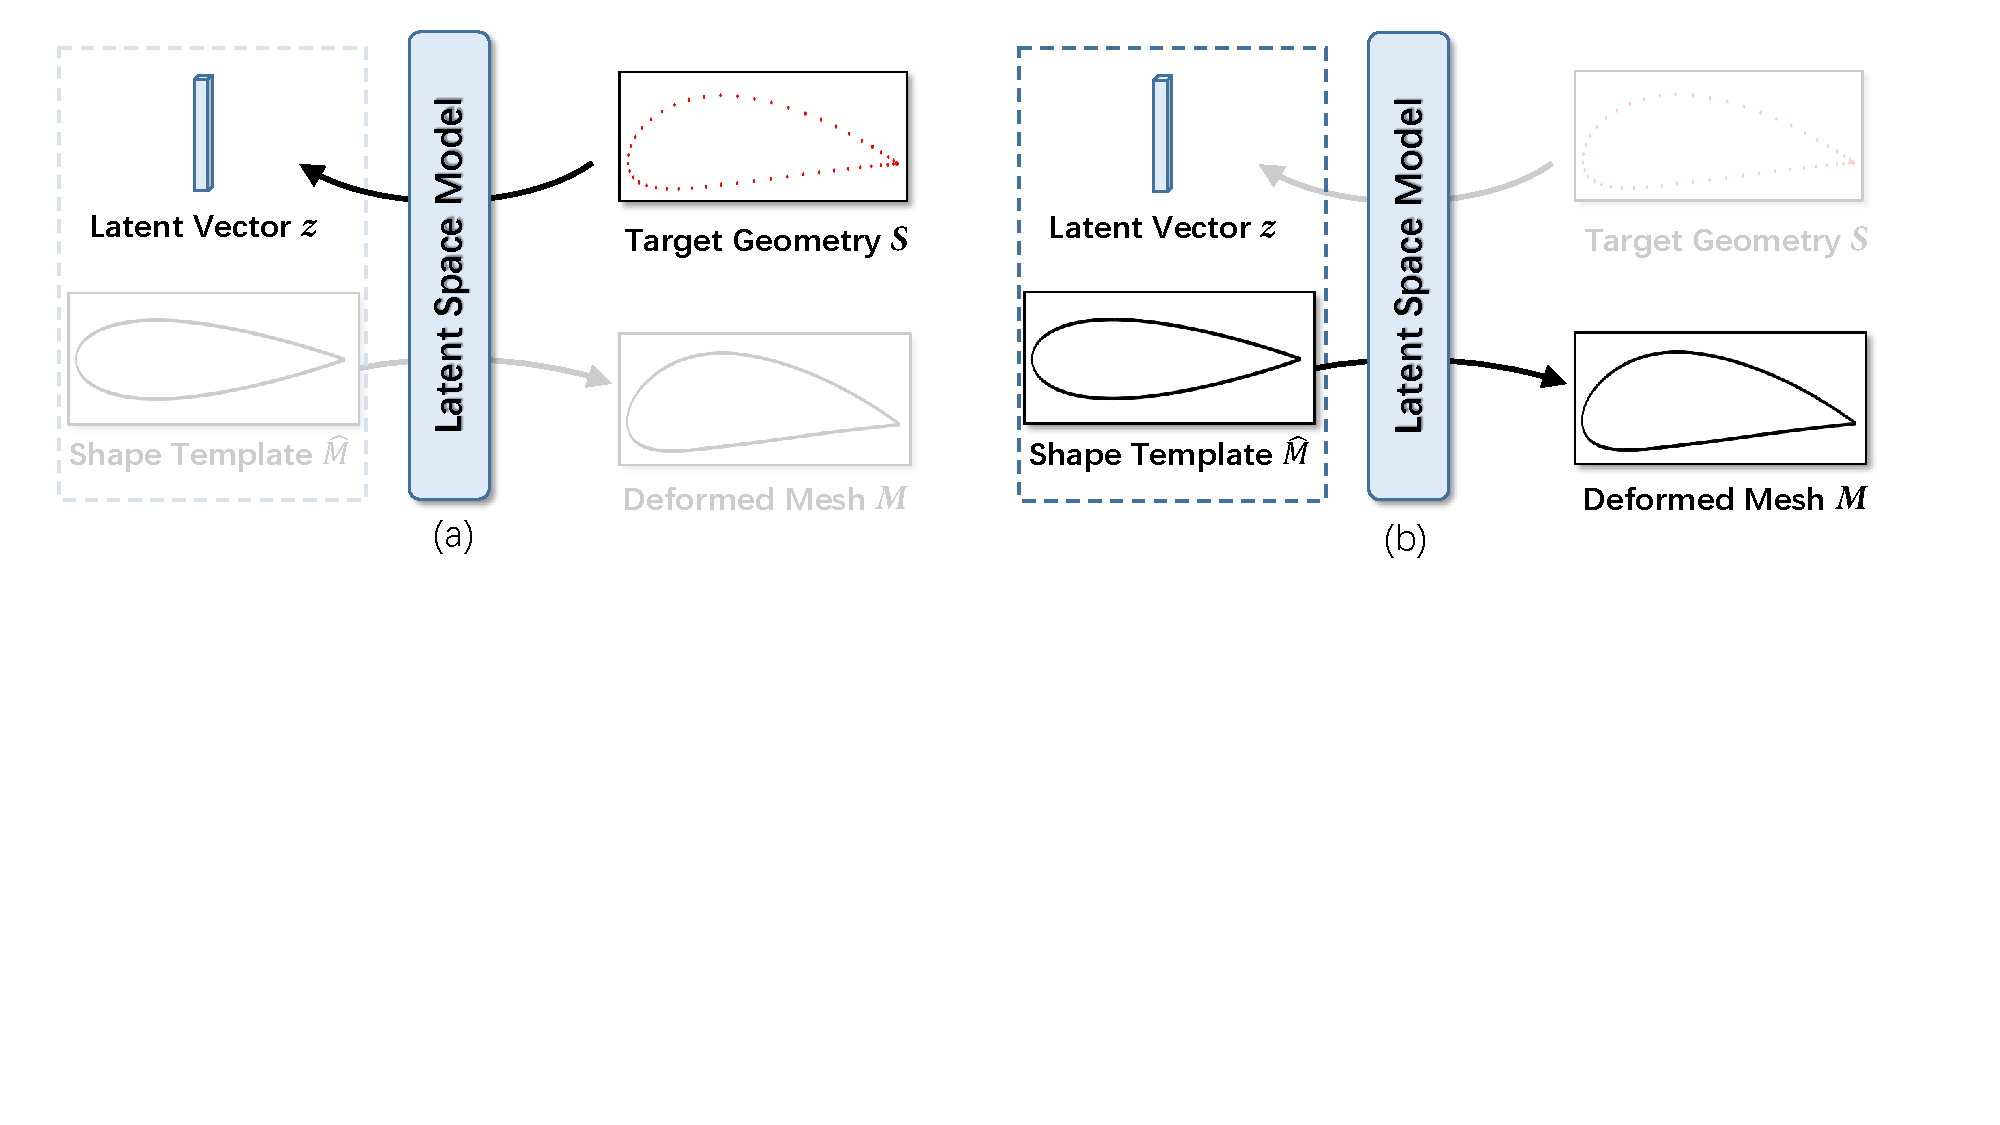
\includegraphics[width=1\linewidth]{chapter4/fig/framework_LSM.pdf}
    \end{center}
    \caption{
        \small The framework of LSM. It first encodes the target geometry into a latent vector, as shown in (a), and then decodes it into a deformation of the shape template, as shown in (b). The latent vector $\bv$ parameterizes the target geometry.
    }
    \label{ch4:fig:framework_LSM}
\end{figure}

\begin{figure}[th]
    \begin{center}
        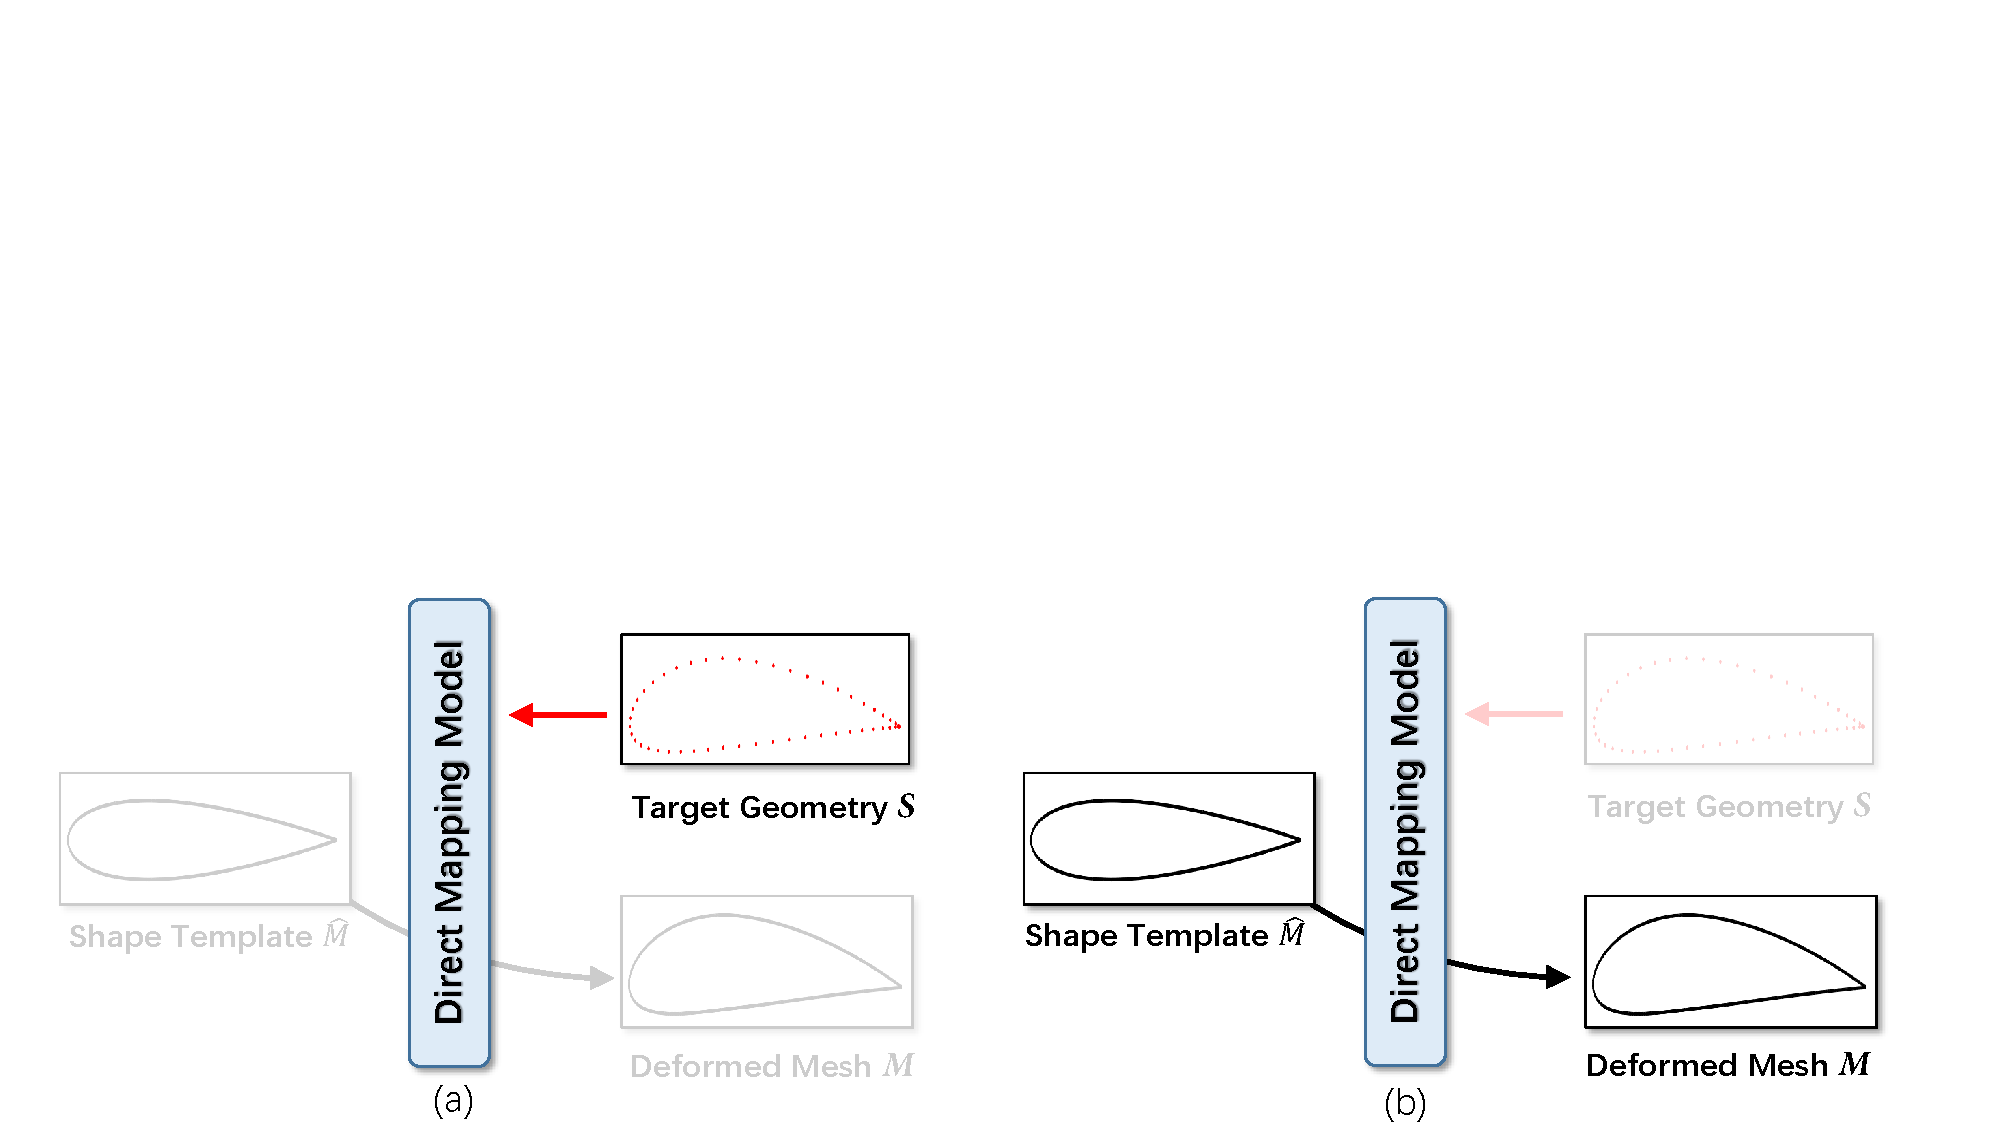
\includegraphics[width=1\linewidth]{chapter4/fig/framework_DMM.pdf}
    \end{center}
    \caption{
        \small The framework of DMM. DMM first learns to fit the target geometry following Eq.\ref{ch4:eq:agmin_g_phi}, as shown in (a). Then the model reconstructs the same geometry by deforming the shape template, as shown in (b). The trainable weights $\Phi$ of DMM parameterize the target geometry.
    }
    \label{ch4:fig:framework_DMM}
\end{figure}

\subsection{The Latent Space Model (LSM)}
LSM relies on the auto-decoder structure \cite{ai.Tan1995,ai.Park2019c} and is trained jointly with the latent space on the collected geometries that belong to a same category (e.g. 2D airfoils). It maps a CFD mesh built on the template airfoil conditioned on a latent vector that parameterizes the target geometric information as
\begin{align}
    f_{\Theta} : \mathbb{R}^d \times \mathbb{R}^D \rightarrow \mathbb{R}^D \; , \label{ch4:eq:map_lsm} \\
    \mathbf{\delta v} = f_{\Theta}(\bz, \hat{\bv}) \; , \nonumber
\end{align} 
where $D$ is the data dimension of CFD mesh, $d \ll D$, and $\bz\in \mathbb{R}^d$ is the low-dimensional latent parameterization. $\Theta$ represents the weights that control LSM $f$. 

During training, a training dataset of $T$ airfoils $S_1,\ldots,S_T$ is collected which only contains sampled surface points. The auto-decoding approach is used to optimize the weights $\Theta$ and the latent vectors that parameterize each training data $\textbf{z}_1,\ldots,\textbf{z}_T$. The training objective writes
%
\begin{align}
\Theta^*,\bZ^* &=  \argmin_{\Theta,\bz_1,\ldots,\bz_T} \sum_{t=1}^T \cL(f_{\Theta}(\bz_t, \hat{\bv}^S), f_{\Theta}(\bz_t, \hat{\bv}^V), S_t) \; ,
\label{ch4:eq:argmin_f_z_theta}
\end{align}
%
where $\cL$ is a loss function that is small when $f_{\Theta}(\bz_t, \hat{\bv}^S)$ yields a deformed airfoil that is geometrically identical to $S_t$, and $f_{\Theta}(\bz_t, \hat{\bv}^V)$ generates a CFD mesh $M$ that possess satisfactory quality. As a result, the optimal $\bz_t^*$ corresponds to a low-dimensional parameterization of $S_t$. 

We use the Chamfer Distance \cite{ai.Barrow1977}, denoted as $\cL_{CD}(V^S, S)$, to measure the geometric difference and the regularization loss, denoted as $\cL_{reg}(V^V)$, to preserve the quality of the computational mesh. Additionally, we apply a constraint on the norm of $\bz$ to ensure the smoothness of the learned latent space.
Therefore, we have the overall training objective that writes
\begin{align}
\cL(V^S, V^V, S) = \cL_{CD}(V^S, S) + w_{reg}\cL_{reg}(V^V) + w_{\bz}\left|\left|\bz\right|\right|^2 ,
\end{align}
where $w_{reg}$ and $w_{\bz}$ are the balancing weights.

At inference time, given a target geometry $S$ and the frozen weights $\Theta^*$, the latent parameterization vector $\bz^*$ is obtained by optimizing the following problem,
%
\begin{align}
\bz^* &=  \argmin_{\bz} \cL(f_{\Theta}(\bz, \hat{\bv}^S), f_{\Theta}(\bz, \hat{\bv}^V), S) \; .
\label{ch4:eq:agmin_f_z}
\end{align}
%
Then the output CFD mesh is obtained by forwarding $\bz^*$ again as $M=\{\{f_{\Theta}(\bz^*, \hat{\bv}^S), f_{\Theta}(\bz^*, \hat{\bv}^T)\}, \hat{E}\}$. 

\subsection{The Direct Mapping Model (DMM)}
DMM is a feed-forward neural network dedicated to map the template airfoil to a single target, which writes
\begin{align}
    g_{\Phi} : \mathbb{R}^D \rightarrow \mathbb{R}^D \; , \label{ch4:eq:map_dmm} \\
    \mathbf{\delta v} = g_{\Phi}(\hat{\bv}) \; , \nonumber
\end{align} 

Unlike LSM, which uses an auto-decoder model and $T$ exclusive latent vectors to parameterize $T$ shapes of the same category, DMM requires $T$ neural networks $g_{\Phi_1}, g_{\Phi_2},\ldots, g_{\Phi_T}$ for $T$ template-to-target geometry mappings.
In DMM, the geometric information is embedded in the model itself and the model's weights parameterize the target geometry without producing an explicit vector as design variables. However, DMM does not have a training process or a requirement for a large amount of data. During inference, $\Phi$ is randomly initialized and then optimized with respect to the target airfoil $S$ to solve the following problem.
\begin{align}
\Phi^* &=  \argmin_{\Phi} \cL(g_{\Phi}(\hat{\bv}^S), g_{\Phi}(\hat{\bv}^V), S) \; .
\label{ch4:eq:agmin_g_phi}
\end{align}

DMM's loss function is similar to LSM's loss function, but without the constraint on the latent space, which writes
\begin{align}
\cL(V^S, V^V, S) = \cL_{CD}(V^S, S) + w_{reg}\cL_{reg}(V^V).
\end{align}

%%%%%%
\subsection{The Regularization for Quality-Preserved Mesh Deformation}
The regularization loss guarantees that all points sampled as $\hat{V}^V$ move in accordance with the changing airfoil geometry to maintain the computational mesh quality inherent in the user-defined CFD mesh that is built on the template airfoil. This quality is reflected in quantitative metrics, such as cells' skewness, orthogonality, and aspect ratio, as well as the mesh's ability to represent the underlying physics~\cite{aa.Knupp2007}.
To this end, we characterize the computational mesh as a discrete sample of a continuous 2D elastic material which is framed by the fixed computational boundaries (typically the inlet/outlet patches) and the deformable airfoil surface.
Mesh quality can degrade due to non-rigid distortion, which changes the angles and edge length ratios within the mesh cells. 
Deformation of computational boundaries can lead to incorrect boundary conditions and hinder the use of generated meshes in downstream software.
To address these issues, we formulate the regularization loss as the sum of two terms, namely $\cL_{dist}$ and $\cL_{def}$, to minimize non-rigid distortion across the entire mesh and the deformation of fixed patches:
\begin{equation}
    \cL_{reg} = \cL_{dist} + \cL_{def}\;\;.
\end{equation}

To formulate $\cL_{dist}$, we define an energy function $\mathbb{E}$ that quantifies the total non-rigid distortion as the squared Frobenius norm of the infinitesimal strain tensor, which writes
\begin{align}
    \begin{split}
        \mathbb{E} &:= \frac{1}{2} \sum_{i=1}^{|V^V|} \left|\left| \nabla \delta \bv^V_i + (\nabla \delta \bv^V_i)^T \right|\right|_F^2  \\
        &\;= \frac{1}{2} \sum_{i=1}^{|V^V|} \left\{ 
        \left|\left| \frac{\partial \delta v^V_{x,i}}{\partial x} \right|\right|^2 + 
        \left|\left| \frac{\partial \delta v^V_{x,i}}{\partial y} \right|\right|^2 + 
        \left|\left| \frac{\partial \delta v^V_{y,i}}{\partial x} \right|\right|^2 + 
        \left|\left| \frac{\partial \delta v^V_{y,i}}{\partial y} \right|\right|^2 \right\} \;\;,
    \end{split}
\end{align}
where the displacement of a single vertex $\delta \bv^V_i = (\delta v^V_{x,i}, \delta v^V_{y,i}) \in \mathbb{R}^2$. Then we investigate the following formula
\begin{equation}
    - \sum_{i=1}^{|V^V|} \left\{
    \frac{\partial^2 \delta v^V_{x,i}}{\partial x^2} +
    \frac{\partial^2 \delta v^V_{x,i}}{\partial y^2} +
    \frac{\partial^2 \delta v^V_{y,i}}{\partial x^2} +
    \frac{\partial^2 \delta v^V_{y,i}}{\partial y^2}
    \right\} \;\;.
    \label{ch4:eq:avm_internal_step}
\end{equation}
Since $\delta \bv_i = \bv_i - \hat{\bv}_i$ and $\partial ^2 \hat{\bv}_i / \partial x^2 = \partial ^2 \hat{\bv}_i / \partial y^2 = 0$, Eq.\ref{ch4:eq:avm_internal_step} can be rewritten as
\begin{equation}
    F := - \sum_{i=1}^{|V^V|} \left\{
    \frac{\partial^2 v^V_{x,i}}{\partial x^2} +
    \frac{\partial^2 v^V_{x,i}}{\partial y^2} +
    \frac{\partial^2 v^V_{y,i}}{\partial x^2} +
    \frac{\partial^2 v^V_{y,i}}{\partial y^2}
    \right\} \;\;.
\end{equation}
$F=0$ for $\forall i$ when $\bv = \hat{\bv}$, which is the Euler-Lagrange equation of $\mathbb{E}$ and is the sufficient and necessary condition of which the user-defined template CFD mesh is a stationary point on $\mathbb{E}$'s energy landscape. $\cL_{dist}$ is then defined to induce local cell structures in the generated computational mesh to resemble those in the template, so as to prevent the creation of meshes with serious issues such as negative-volume cells and severely non-orthogonal issues. The desired mesh properties embedded in the template mesh, including cell aspect ratio, skewness, and orthogonality, are also preserved as much as possible.
$\cL_{dist}$ is defined as
\begin{equation}
    \cL_{dist} := \sum_{i=1}^{|V^V|} \left\{
    \left|\left| \frac{\partial^2 v^V_{x,i}}{\partial x^2} \right|\right|^2 + 
    \left|\left| \frac{\partial^2 v^V_{x,i}}{\partial y^2} \right|\right|^2 + 
    \left|\left| \frac{\partial^2 v^V_{y,i}}{\partial x^2} \right|\right|^2 + 
    \left|\left| \frac{\partial^2 v^V_{y,i}}{\partial y^2} \right|\right|^2
    \right\} \;\;.
\end{equation}
Thanks to the full differentiation of LSM and DMM, the PDE terms can be easily computed analytically through auto-differentiation.

$\cL_{def}$ measures the deformation near the boundaries, which writes
\begin{equation}
    \cL_{def} := \sum_{j=1}^{|V^{fix}|} \left|\left| \delta \bv^{fix} \right|\right|^2 \;\;,
\end{equation}
where $V^{fix}=\{\bv^{fix}_1,\bv^{fix}_2,\ldots,\bv^{fix}_k\}$ is a set of sampled points on or closed to the computational boundaries (i.e. inlet/outlet patches) and any other specified fixed patches, and is a subset of $V^V$.

%%%%%%
\subsection{Discussions on LSM and DMM}
\label{ch4:sec:discussion_lsm_dmm}
\subsubsection{The Commonness of LSM and DMM}
LSM and DMM learn continuous mappings between coordinate spaces. The sampling strategy of $V^S$ and $V^V$ can be independent of any specific CFD mesh, or can use a CFD mesh to sample but to generalize to any other discrete sampling in the continuous space.
This enables both models to infer with various CFD meshes after optimizing $\Theta$ or $\Phi$ without any adaptation.
Fig.\ref{ch4:fig:infer_different_templates} demonstrates the reconstruction results of both models inferred with different template meshes.

\begin{figure}[!htb]
    \begin{center}
        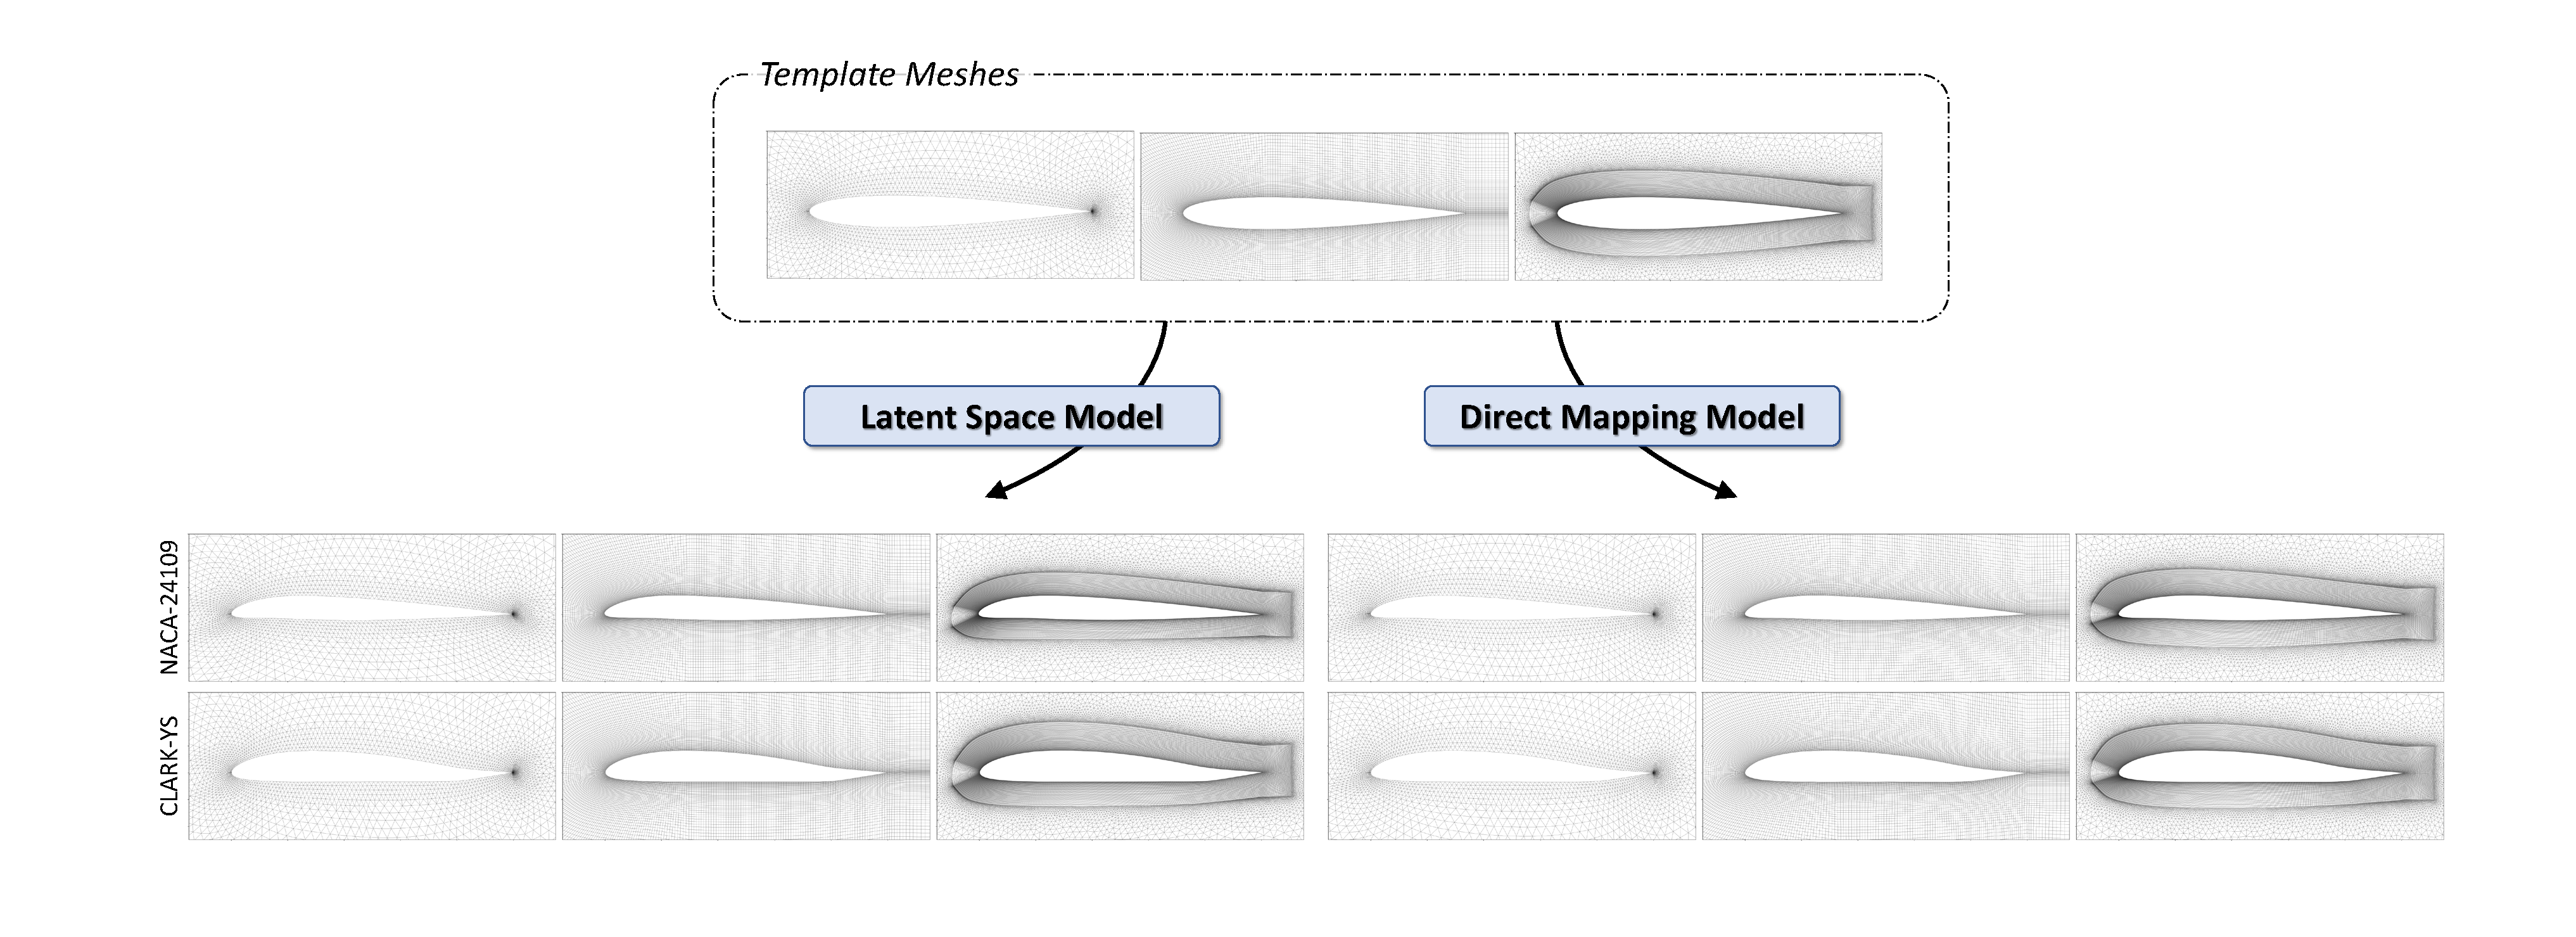
\includegraphics[width=1\linewidth]{chapter4/fig/infer_different_templates.pdf}
    \end{center}
    \caption{
        \small Both optimized LSM and DMM can infer various template CFD meshes accurately without requiring any adaptations.
    }
    \label{ch4:fig:infer_different_templates}
\end{figure}

Meanwhile, $\cL_{reg}$ incorporates the mesh deformation into the parameterization models, eliminating the need for an additional postprocessing module. It does not introduce sensitive hyperparameters to tune or manual configurations. Additionally, compared to RBF-based methods and spring analog methods, $\cL_{reg}$ does not need to solve a huge linear system of vertices. It is also more computationally efficient than IDW-based methods. Let $N^*$ and $M^*$ be the numbers of vertices of the geometry surface and the computational mesh for a specific CFD mesh, respectively. The number of sampled $V^V$ is $M$, and $M<<M^*$. The complexity of $\cL_{reg}$ is $\cO(M)$ during training and is none during inference, whereas it is $\cO(N^*M^*)$ for IDW-based methods for every deformation.

\begin{figure}[!tb]
    \begin{center}
        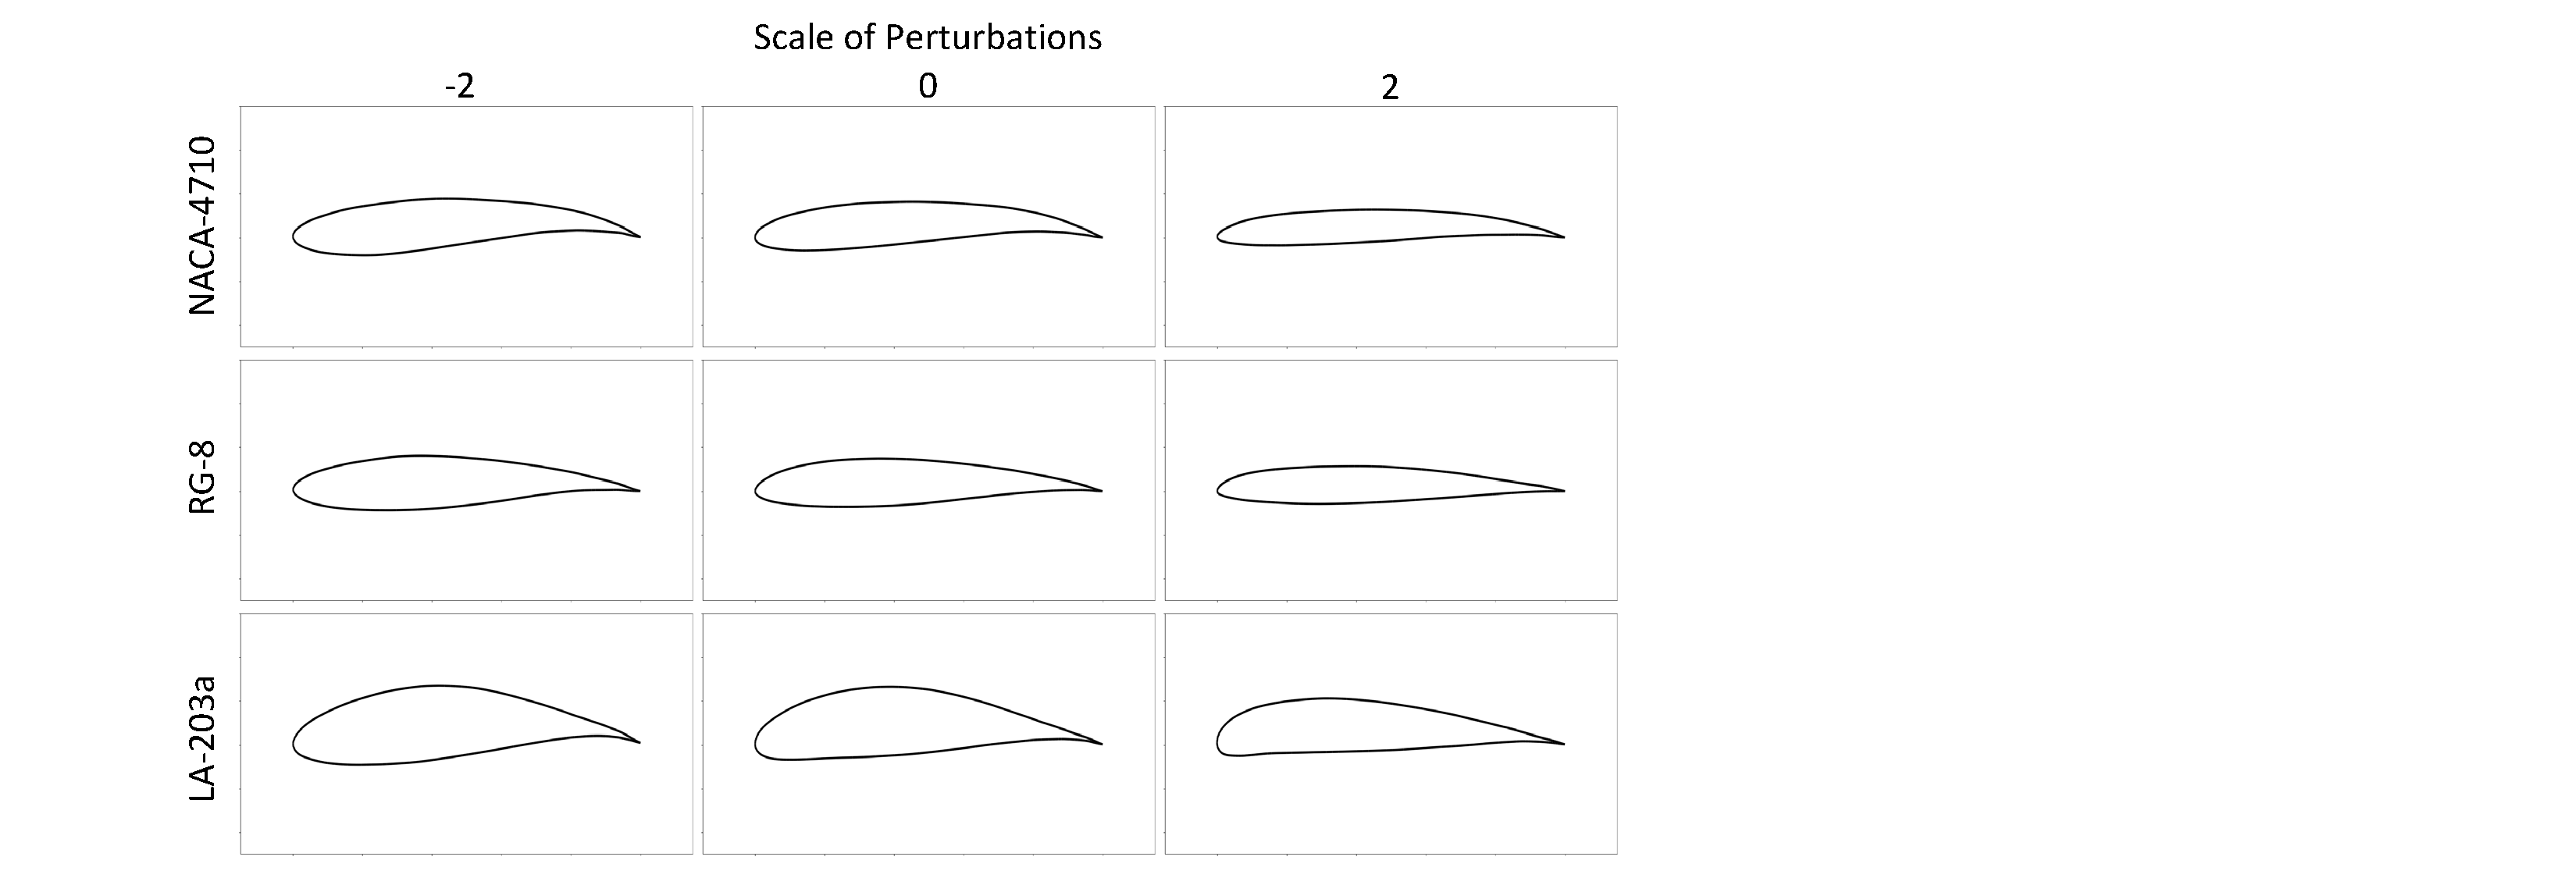
\includegraphics[width=0.75\linewidth]{chapter4/fig/lsm_sample.pdf}
    \end{center}
    \caption{
        \small The novel airfoils sampled in LSM's learned latent space by perturbing the latent parameterization vectors of existing profiles with the sampling method proposed by \citet{ai.Shen2021b}.
    }
    \label{ch4:fig:lsm_sample}
\end{figure}
\begin{figure}[!tb]
    \begin{center}
        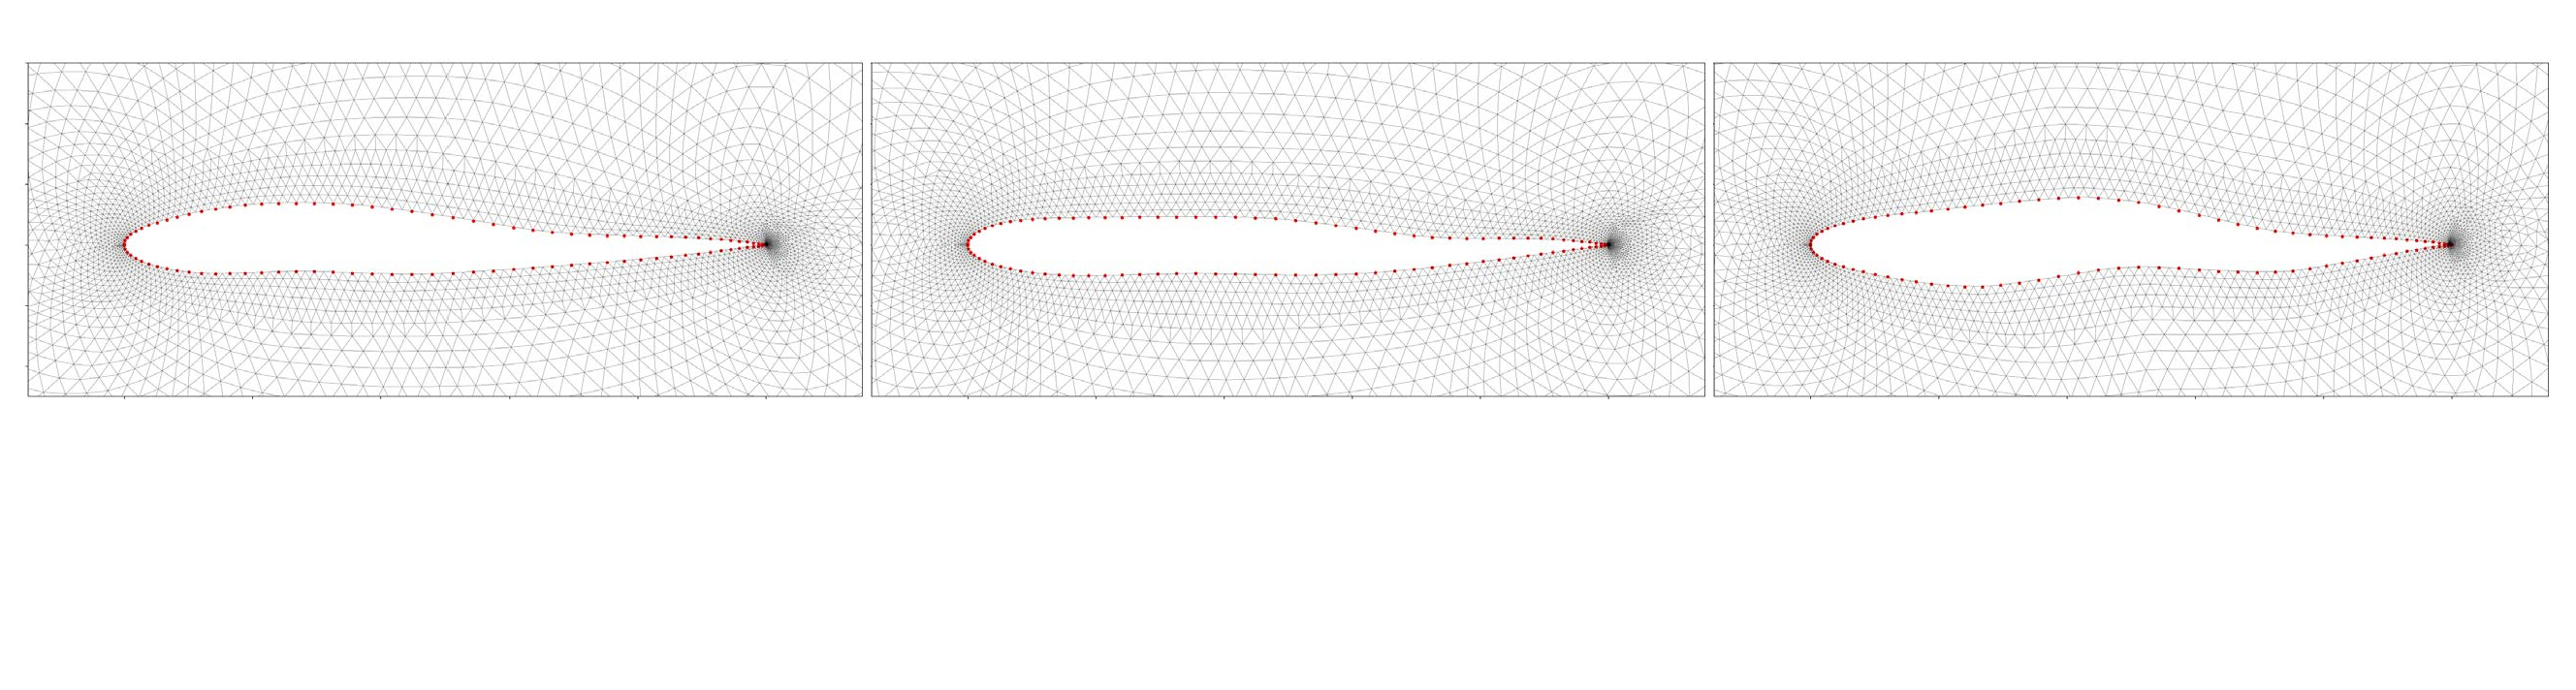
\includegraphics[width=1\linewidth]{chapter4/fig/dmm_various_target.pdf}
    \end{center}
    \caption{
        \small The reconstruction results of DMM that parameterize the randomly deformed airfoils. The true geometries of the targets are represented by the red dots.
    }
    \label{ch4:fig:dmm_random_reconstruct}
\end{figure}

\noindent\textbf{The Unique Properties of LSM}

LSM and DMM have different properties due to their different optimization strategies.

The latent space jointly trained with LSM's network embeds rich geometric information from the training data. Novel shapes generated by LSM interpolate the design space defined by the training set and inherit the geometric prior. When perturbing $\bz$ of an existing airfoil slightly, one can obtain another novel airfoil instead of any non-airfoil shape. This property has two major benefits. First, LSM can be used as a novel data sampler. Fig.\ref{ch4:fig:lsm_sample} demonstrates the explored novel shapes from existing airfoils by LSM using the sampling-free approach proposed in \cite{ai.Shen2021b}. Second, when performing shape optimization with LSM, we can use fewer explicit geometric constraints to ensure the validity of the optimized result, such as maintaining the surface smoothness, object scale and the special structures commonly appeared among the training data.

LSM is an upgraded version of the model proposed in Wei et al. \cite{aa.Wei2023} with a simplified structure and regularization loss, resulting in less computational time and memory consumption during both training and inference.

\noindent\textbf{The Unique Properties of DMM}

DMM is a lightweight model suitable for a case study of a specific geometry of interest. It does not require a training dataset, which is not always available. Optimizing DMM takes $4-6s$ for 2D airfoil cases. Meanwhile, DMM encodes the geometric information of a single object, which allows for more geometric freedom and the ability to deform the template shape into various geometries. Fig.\ref{ch4:fig:dmm_random_reconstruct} demonstrates that DMM can reconstruct and parameterize randomly twisted shapes from the template airfoil NACA-0012. Using DMM as the parameterization model, shape optimization can explore and develop novel structures.

\subsection{Implementation}
The LSM and DMM are implemented using the Pytorch deep learning framework \cite{ai.Paszke2019}. LSM is a four-layer multi-layer perceptron (MLP) network with a $256$-dimensional latent space. The activation function of each latent MLP layer is a weighted sum of ReLU \cite{ai.Fukushima1975} and SIREN \cite{ai.Sitzmann2020}, which enables accurate shape deformation and the computation of second-order partial derivatives. LSM is trained on $2648$ airfoils, including $1442$ data of various foil series collected from the UIUC airfoil dataset \cite{aa.Selig1996} and the remaining airfoils being random NACA 4-digit or 5-digit profiles. The training uses the Adam optimizer \cite{ai.Kingma2015b} with an initial learning rate of $10^{-4}$ for 20 epochs, which costs $175s$.
During inference, the latent vector $\bz$ is optimized with the Adam optimizer with at maximum $1000$ iterations.

DMM uses a similar network structure as LSM, but with only two latent layers. During inference, the Adam optimizer solves Eq.\ref{ch4:eq:agmin_g_phi} with $600$ iterations.

\begin{figure}[tbh]
    \begin{center}
        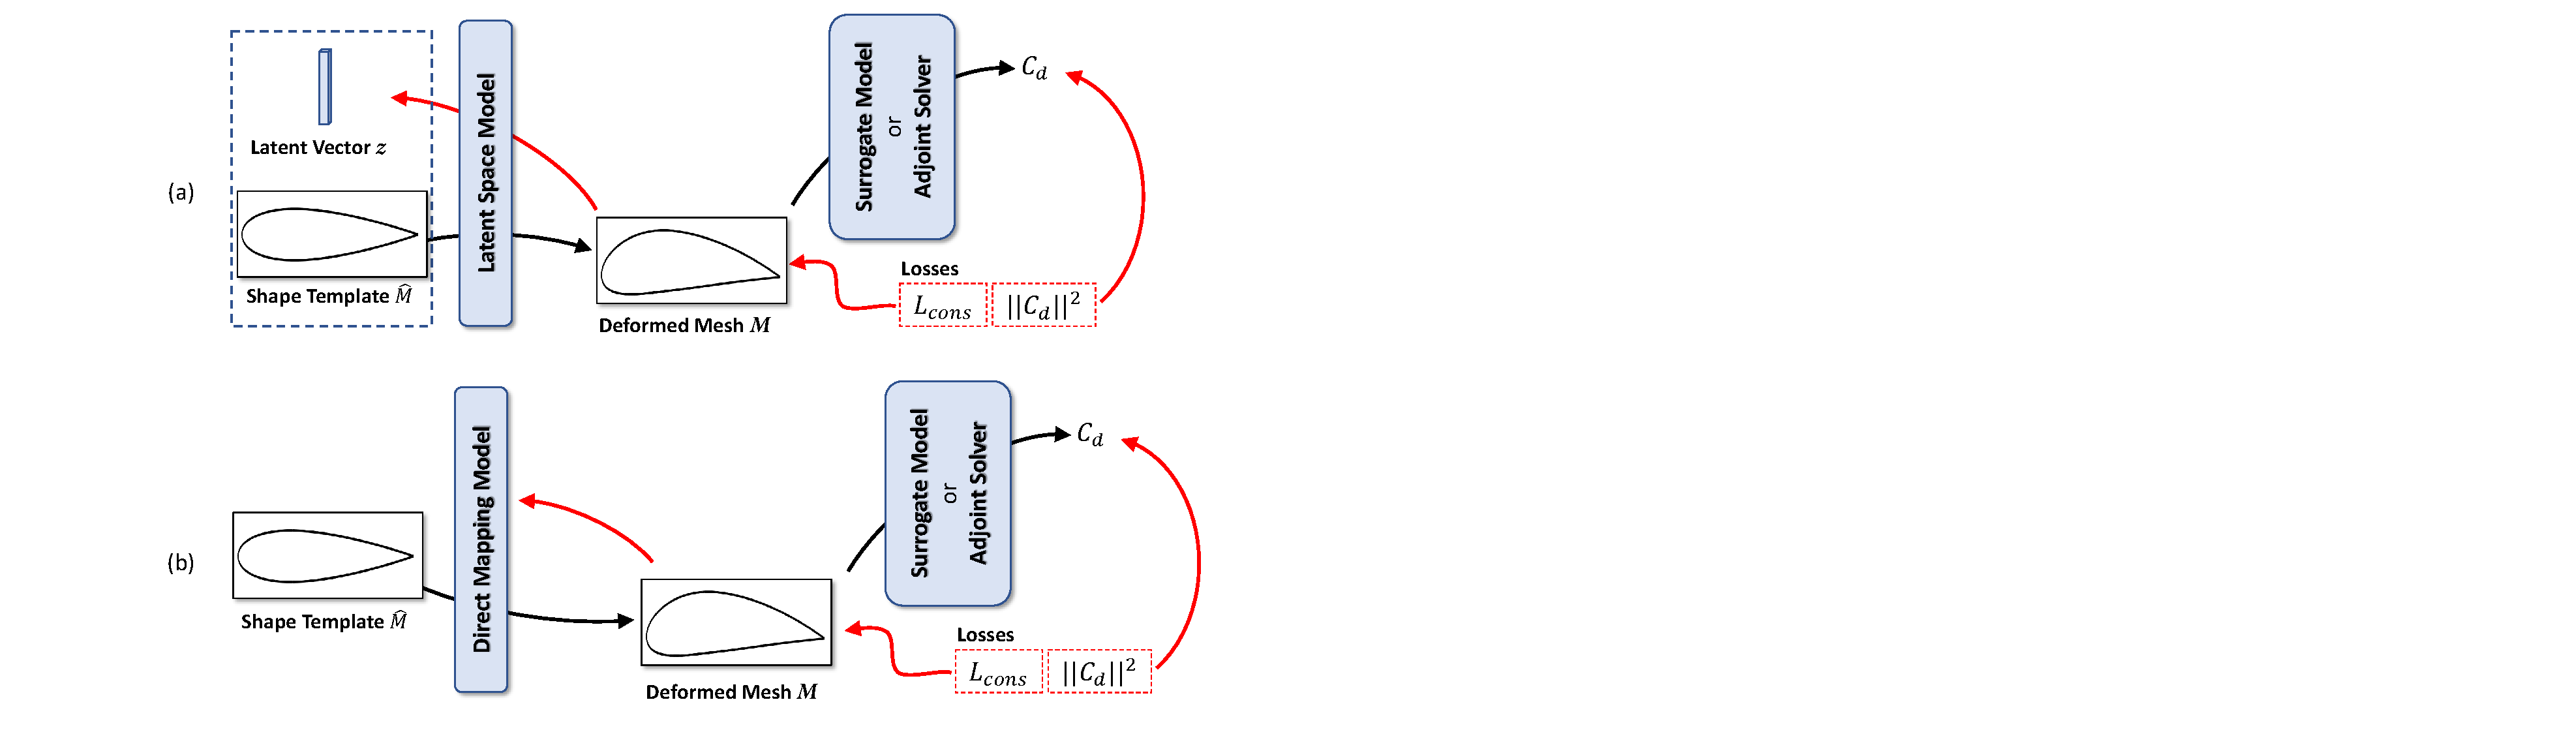
\includegraphics[width=1\linewidth]{chapter4/fig/framework_optim.pdf}
    \end{center}
    \caption{
        \small The shape optimization frameworks with the use of (a) LSM and (b) DMM. The surrogate model or the adjoint solver is appended after the inferred meshes. Red paths illustrate the gradient flows in the pipeline.
    }
    \label{ch4:fig:framework_optim}
\end{figure}

\subsection{Fully Differentiable Frameworks for Shape Optimization}
In this paper, we use LSM and DMM parameterization models to provide an example of solving the ADODG Case 1 optimization problem with a gradient-based solution. The objective is to minimize the drag coefficient of the NACA-0012 airfoil in a transonic flow (Ma=0.85) at zero angle-of-attack.

To perform aerodynamic shape optimization, we need to couple LSM or DMM with a downstream evaluation module (denoted as $h$), which can be either a differentiable surrogate model (such as the GCNN network~\cite{aa.Baque2018}) or an adjoint solver (such as SU2~\cite{aa.Economon2016}), to evaluate the performance of the current design. For example, the evaluate of drag can be writted as
\begin{equation}
    C_d = h(M)\;,
\end{equation}
where $M=\{\{\hat{V}^S+\Delta V^S, \hat{V}^V+\Delta V^V\}, \hat{E}\}$ is inferred by $f_{\Theta}$ or $g_{\Phi}$.
The geometric constraints $\cL_{cons}$ can be directly calculated from $M$ and then applied to $M$. The overall pipelines are illustrate in Fig.\ref{ch4:fig:framework_optim}. The shape optimization objectives are written as
\begin{align}
    \text{for LSM: }&\;\;\; \bz^* =   \argmin_{\bz} \left( \left|\left|C_d\right|\right|^2 + \cL_{cons}(M(\hat{V} + f_{\Theta}(\hat{M},\bz))) \right)\; ,\\
    \text{for DMM: }&\;\;\;  \Phi^* =   \argmin_{\Phi} \left( \left|\left|C_d\right|\right|^2 + \cL_{cons}(M(\hat{V} + g_{\Phi}(\hat{M},\bz))) \right)\; .
\end{align}

The gradients from the surrogate model or the adjoint solver, as well as the constraints, will be backpropagated to the latent code of LSM or to the weights of DMM. The output shapes are then manipulated by applying an optimizer to update the learnable parameters.